%!TEX root = ../template.tex

\chapter{System Model and Design Options}
\label{cha:system_model_and_design_options}

In this chapter we provide an overview of the system model and implemented architecture along with all of its components. It is explained how all component interact with each other and each component purpose and how they work.

It is also explained how the different security features are implemented into the system in order to provide a secure overall system and achieve the contributions planned for this thesis.

(...)

In section \ref{sec:threat_model_and_security_properties} we describe the basic security assumptions need for our system to work securely. The threat model is a very important part of any security related project as it provides a clear overview of what attacks the system is able to protect against, presents the trustability chain and \gls{TCB} as well as what components and  security properties are out of scoped and not addressed in the project.
Sections \ref{sec:system_model} and \ref{sec:proposed_architecture} presents an high level view of the system model and implemented architecture of the system. Then, in section \ref{sec:operations_supported} and \ref{sec:logging_and_auditing} we expose the application specific operations supported and auditing services of the system.

Finally, as always, section \ref{sec:chapter3_summary} we summarise all the findings and provide a clear transition into chapter \ref{cha:elaboration_plan}, which will present all implementation specific details performed to achieve the described system.

\section{Refinement of Objectives and Contributions} % (fold)
\label{sec:refinement_of_objectives_and_contributions}

The goal of this dissertation as explained on chapter \ref{cha:introduction}, is the design, development and validation with experimental evaluation of a secure in-memory storage (based on a "key-value" model), supported by a hardware-enabled trust computing base.

Regarding the security assumptions, the solution will provide: (i) hardware-isolated in-memory processing engine, designed as a hardware-isolated container facility, enclaved within the Intel-SGX protection guarantees; (ii) hardware-isolated communication endpoints for client access, providing TLS tunnelling with strong TLS 1.3 endpoint encryption parameterisations and support for mutual client/server authentication, and (iii) privacy-enhanced operations to be directly processed on encrypted data sets in memory. The former facility is particularly interesting to combine the possibility to manage protected memory for small data sets and also searchable encrypted data sets that are far larger than the protected memory limits imposed by the SGX memory mapping facility. Furthermore, the solution will target main data structures commonly use fine-grained data items that can include pointers, complex composite types and keys, which do not match well with the coarse-grained paging of the SGX memory extension technique.

In the next subsections we will align the implementation ideas starting by refining the circumvention of limitations in SGX and the threat model assumptions to address our solution.

\subsection{\gls{SGX} Limitations Refinement}
\label{ssec:sgx_limitations_refinement}

Section \ref{ssec:circumvention_of_sgx_limitations} describes in detail the limitations of \gls{SGX}. In our approach we will intend to design a solution that can be leveraged from conventional reference KVS technology, giving the possibility to manage small datasets but also larger datasets (directly mapped in non-protected memory). To circumvent the problem our solution must combine the possibility to use the internal capabilities native to SGX with the possibility of supporting operations managing datasets encrypted in memory, with such operations executed directly over encrypted data. This facility will be provided by the use of partial homomorphic encryption constructions, with data initially encrypted and submitted to the key-value-store solution with cryptographic keys only managed in the client side. Our solution will be designed in order to be possible the support for fine-grained key-value encryption, driven form the application requirements. Our target is the support of a variety of operations provided in a typical KVS API, taking REDIS as the reference solution and in order to support a considerable number of queries currently used by many REDIS-supported applications.

\section{Threat Model and Security Properties}
\label{sec:threat_model_and_security_properties}

The ensure basic security system, we need to work within a few key parameters:
 
\textbf{Data Privacy} - Data must remain private to its owner.

\textbf{Data Integrity} - Data must not be compromised, modified or corrupted.

\textbf{Authenticity} - Data and system interactions should be authentic and not spoofed by unauthorised users.

Subsections \ref{ssec:adversarial_model_definition}, \ref{ssec:other_system_assumptions} and \ref{ssec:contermeaseures_for_privacy_preservation} explain under which conditions and assumptions the system will achieve these three main parameters and implement a secure system.

\subsection{Adversarial Model Definition}
\label{ssec:adversarial_model_definition}
	
As the baseline, our threat model will lie on the protection overview stated in SGX’s paper \cite{sgx:7}: \textit{SGX prevents all other software from accessing the code and data located inside an enclave including system software and access from other enclaves. Attempts to modify an enclave’s contents are detected and either prevented or execution is aborted}, which falls in the following adversary model:

\textbf{Isolation by trusted containerisation from malicious code}: The system performs and protects its data from an attacker capable of compromising the system through another application installed on the same system or malicious code existent or injected in the OS or OS hypervisor layers;

\textbf{Privacy protection against insider "Honest but Curious" System Administrators}: The system must be able to protect from an attacker with root access to the machine, with permissions to access and monitor memory-mapped data. This is relevant because we will target our solution as a candidate solution to protect data privacy in a cloud-based key value store solution as a service, preventing data-leakage vulnerabilities exploitable by insider incorrect users or system-administrators.

\textbf{Network Attacks:} All communication to and from the system (supporting client-service operations) should be secure, using proper strong cryptographic parameterisations for TLS 1.3, mutual authenticated handshakes and TLS endpoint executions isolated in SGX-enabled TLS tunnels in communication containers, avoiding attacks against the authentication of the service endpoints, as well as, attacks against the integrity and confidentiality of data flows supporting \gls{REST}/\gls{HTTPS} operations.

\textbf{File system and memory access attacks:} All sensitive data residing outside protected memory should be encrypted and operated in the encrypted form. An attacker can access the physical disks and hardware without the sensitive data being exposed.
	
\subsection{System Assumptions}
\label{ssec:other_system_assumptions}

With the above security baseline considered for the threat model assumptions, the solution must be  resilient to malicious privileged attacks and certain physical attacks. With a controlled and reduced hardware-shielded trust computing base, we want to design a solution that does not rely on the security of operating system managed by cloud providers. Furthermore, our solution must be also resilient to direct conventional physical attacks, such as cold boot attacks, which attempt to retain the DRAM data by freezing the memory chip or even bus probing to sense and to read exposed memory channel between the processor and memory chips. The only weaknesses not covered in our concerns with be the SGX  lack of protection for side-channel attacks.

The system planned has certain assumptions and aspects that are considered to be out of scope for this dissertation:

\begin{itemize}
	\item \textbf{Trusted Client} - The client side is assumed to be completely trusted and correct.
	\item \textbf{\gls{DoS} and \gls{DDoS}} attacks are out of scope.
	\item \textbf{Side Channel Attacks} - It is out of scope any side channel attacks or any related attack not present in \gls{SGX}'s threat model.
	\item \textbf{Physical and Hardware attacks} exploring the \gls{SGX} processing model and its isolation guarantees are out of scope, namely those presented above initially addressed in chapter \ref{cha:related_work}, section \ref{sec:trusted_computing _environments}.
\end{itemize}

\subsection{Countermeasures for Privacy-Preservation}
\label{ssec:contermeaseures_for_privacy_preservation}

Under the described threat model and system assumptions, the system has some measures to achieved the desired security and trustability level.

All instances of the datastore are running in a containerised solution which means that each container is not only isolated from the host but they are also isolated from each other. Data is kept in memory at all times unless persistent disk storage is turned on. Data in main memory is secure when running both in protected and unprotected mode. 

Privacy, integrity and authenticity when running in protected mode are always ensured by the \gls{SGX}'s technology under their threat model and assumptions. But when the system is running in unprotected memory, outside the trusted execution environment, the system will always keep data always encrypted with strong and standard state of the art cryptography algorithms, therefor preserving privacy of data. 

For data integrity preservation, all values are appended with standard checksums calculations and integrity check algorithms. Authenticity is preserved by performing strong and standard cryptographic signing algorithms.

As for the application security, the system provides a secured \gls{API} that only allows authenticated requests and it contains a role based segmentation authorisation with secure and strong passwords and cryptographic keys. This system also applies the principle of least privilege \cite{polp:1} to all actions, where users never have more privileges that they require.

Privacy is also preserved on all communications with the use of the strongest transport layer security algorithms currently available, and established trust between all components with a trusted certificate chain.

\section{System Model} % (fold)
\label{sec:system_model}

The main goal of this project is modelled in figure \ref{fig:system_model_overview}. As shown, the model can be divided in four main components - the \textbf{client}, the \textbf{proxy server}, the \textbf{key-value storage server} and the \textbf{authentication server}.

% \subsection{General Overview}
% \label{ssec:general_overview}

\begin{figure}[htbp]
  \centering{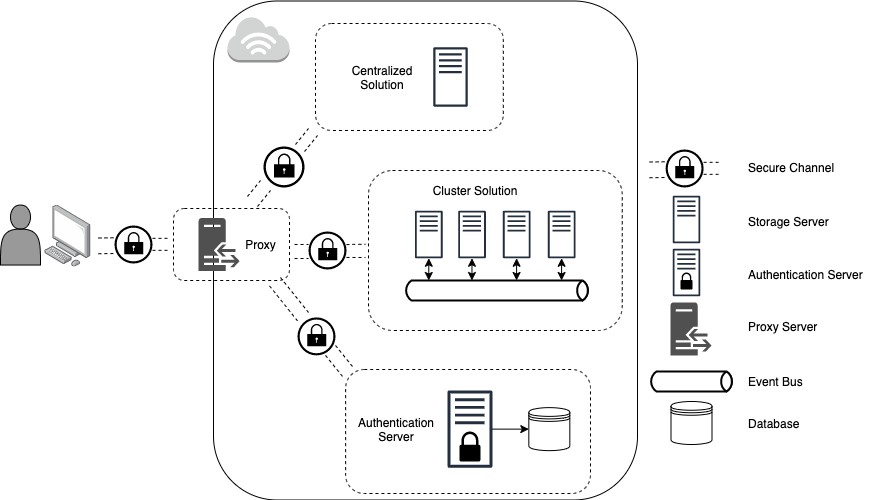
\includegraphics[width=1.0\linewidth]{FinalSystemModel}}%
  \caption{System Model Overview}
  \label{fig:system_model_overview}
\end{figure}

The system complies with the adversary and threat model explained in section \ref{ssec:adversarial_model_definition}. The user is not aware of any implementation details and has seamless interaction with the system despite the architecture and implementation provided by the backend, meaning that all solution expose the same \gls{API} and support an interface as equal as possible to the unprotected version of the key-value store. 

All of the four main components will be explained in the subsections below.

\subsection{Key-Value Storage Server}
\label{ssec:key-value_storage_server}

The storage server is a key-value store meant to hold data required by the user. This data is kept in memory so it allows fast read, writes, updates and deletes.

In this project, there will be two different kinds of storage servers. The \textbf{secured} and \textbf{unsecure} storage server. This nomenclature do not reflect the privacy, integrity and authenticity security problems as they are preserved on both components but it reflects the environment which they will run on.

The \textbf{secure} storage runs on a trusted hardware protected by a secure physical processor present on the host machine. This processor provides the security features that allow for memory to be operated in plain text without breaking privacy or data security.

As for the \textbf{unsecure} storage, it describes a storage service that runs on unprotected memory regions and on untrusted hardware. This means that data must be actively secure by encryption, integrity checks and authentication features in order to provide and preserve privacy.

We must mention that the above system model addresses the replication facilities as leveraged from the Redis solution and tries to offer the same availability conditions as the original Redis service. Both secure and unsecure configurations will provide availability by running replicated Redis instances in a cluster. This availability provided by the replication of Redis instances that can run as cloud service instances (that can be distributed among different cloud providers and geo-replicated datacenters) only offers consistency guarantees under a fail-stop model (not extended to byazntine-fault-tolerance or byzantine intrusion tolerance, that are conditions out of scope of our planned dissertation).

Every Redis instance running on a secure configuration will also provide an API for remote attestation, so their hardware stack and software can be attested by remote parties, to provide trust to the users.

\subsection{Proxy Server}
\label{ssec:system_model_proxy_server}

overview abstracta (sem indicar aspectos tecnicos da implementacao)
visão macro do sistema
	Clientes falam com uma memory KVS que está a correr em cloud, num TEE
	Passam pelo proxy
	Proxy, why? - intermediar acesso ao Redis
Caso seja neutro (nao adicione features)
ajuda caso haja muitas instancias redis espalhadas, assim serve de single point of access para o cliente
filtragem (firewall unica)
overhead extra
single point of failure
(pode ser colmatado caso repliquemos o proxy, mas nao entra no escopo da tese)
Caso seja não neutro (tem features extra)
      (exemplo authentication)
redis tem auth
mas tem que ser configurado individualmente em cada instancia
caso haja muitas, aumenta complexidade  
	
Etc… falar das restantes entidades que vao entrar no sistema

\subsection{Client/Tester}
\label{ssec:clienttester}

\subsection{Authentication Server}
\label{ssec:authentication_server}

\section{Proposed Architecture} % (fold)
\label{sec:proposed_architecture}

\subsection{SaaS/PaaS Infrastructure}
\label{ssec:saas_pass_infrastructure}

\subsection{System Architecture}
\label{ssec:system_architecture}

\subsection{SSL, HTTPS and Certificate Chain}
\label{ssec:ssl_https_certificate_chain}

\section{Operations Supported} % (fold)
\label{sec:operations_supported}

\subsection{Role-Based Authorisation}
\label{ssec:role-based_authorisation}

\subsection{Redis Operations}
\label{ssec:redis_operations}

1. Set
2. Get
3. Set list
4. Get list
5. Set members with score
6. Get members between score

\subsection{Proxy Enabled Operations}
\label{ssec:proxy_enabled_operations}

1. Sum 
2. Subtraction
3. Multiply

\subsection{Attestation}
\label{ssec:proxy_attestation}

\section{Logging and Auditing} % (fold)
\label{sec:logging_and_auditing}

Maybe move this section to implementation

\section{Summary} % (fold)
\label{sec:chapter3_summary}

%% Dissertation Plan Chapters below

\section{System Model Approach} % (fold)
\label{sec:system_model_approach}

The main goal of this project is modelled in figure \ref{fig:syste_model_detailed}. As shown, the model can be divided in three main components - the \textbf{client} which was already defined as trustable, the \textbf{communications} and the \textbf{backend service}. 

\begin{figure}[htbp]
  \centering{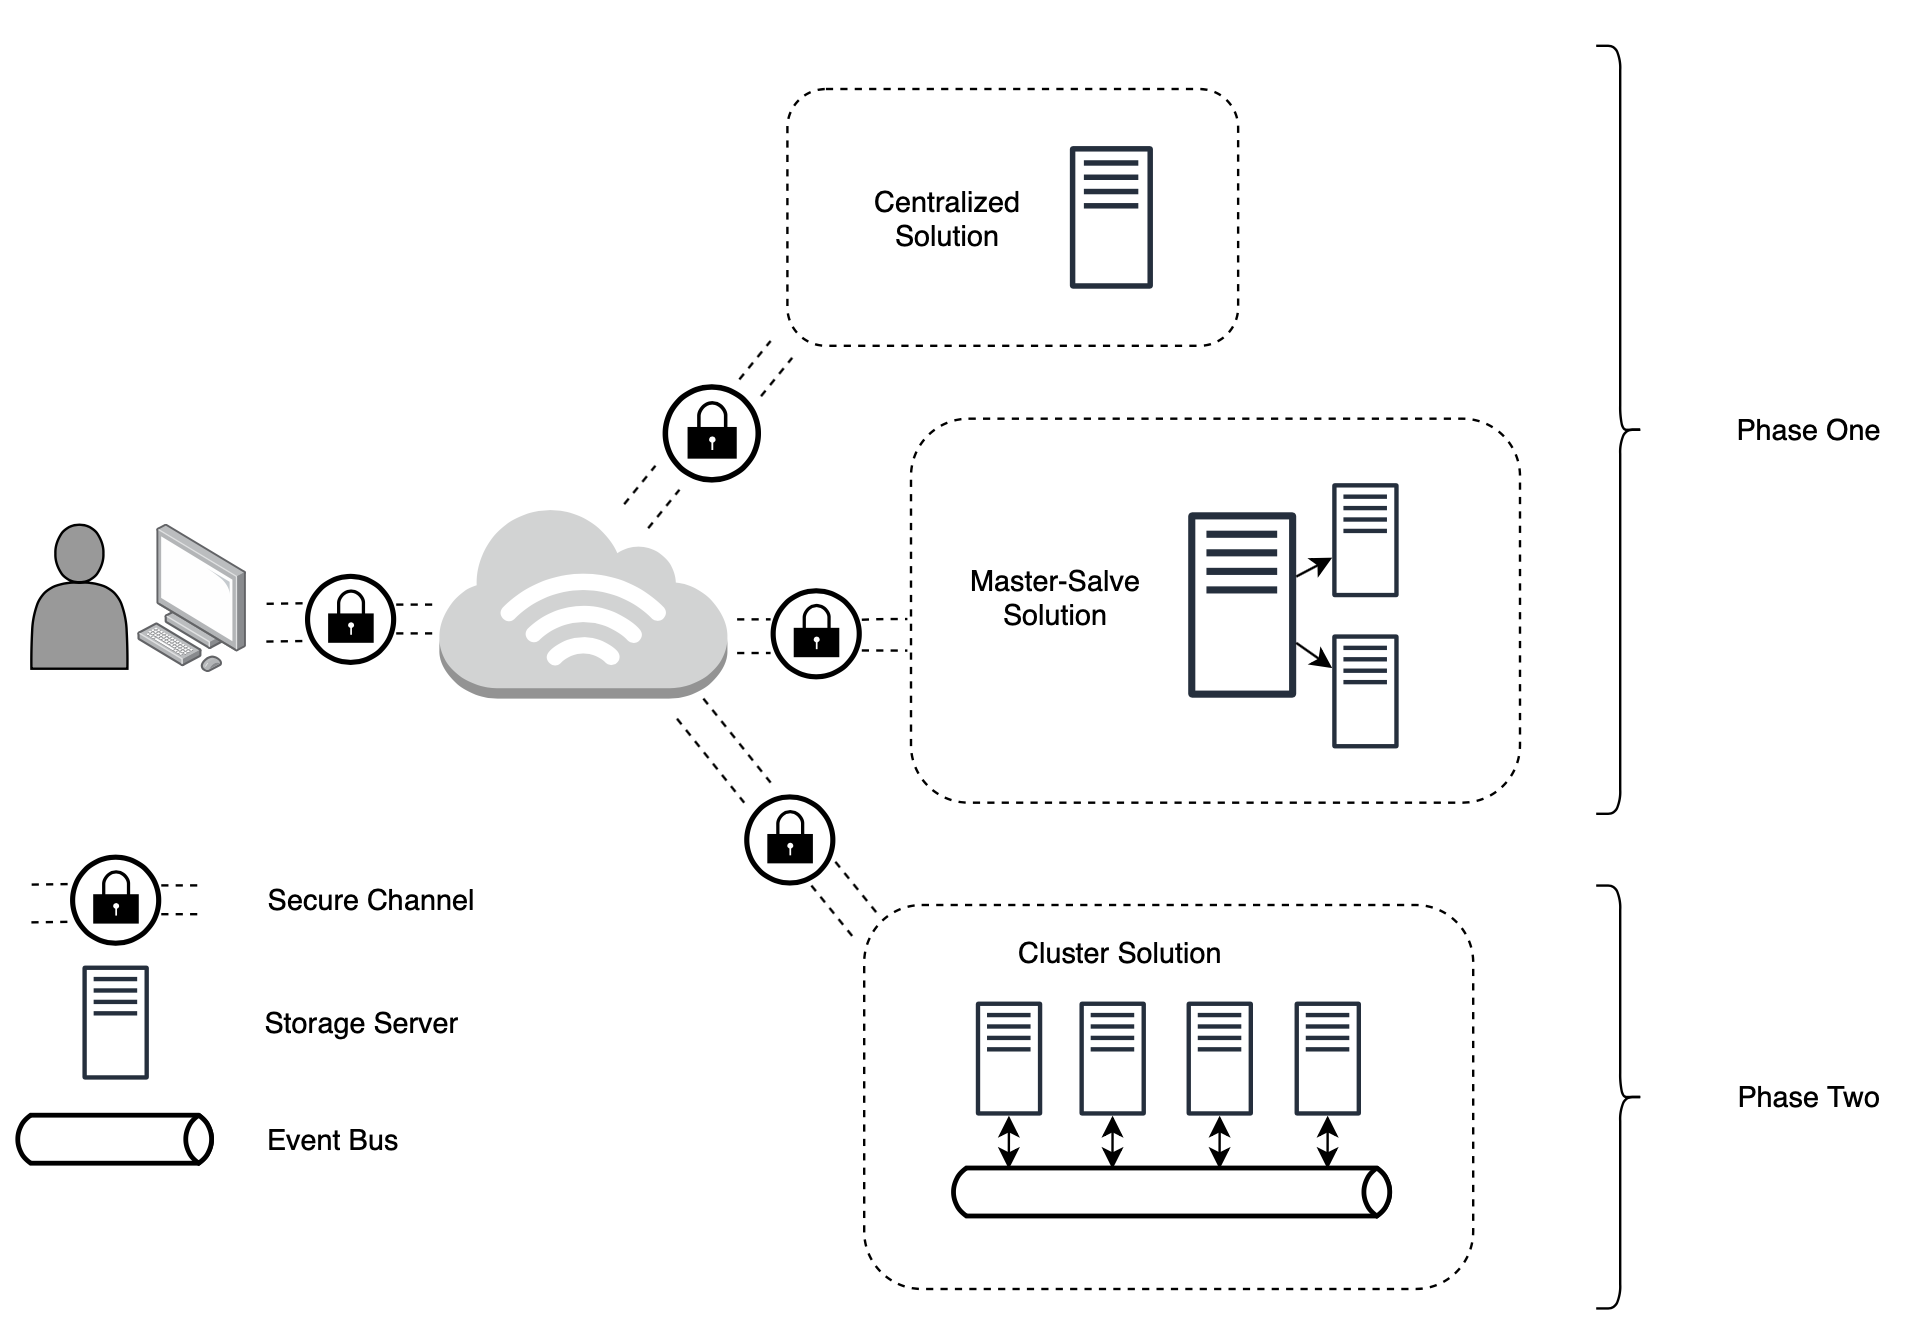
\includegraphics[width=0.9\linewidth]{SystemModelDetailed}}%
  \caption{System Model Details}
  \label{fig:syste_model_detailed}
\end{figure}

The system should comply with the adversary and threat model explained in section \ref{ssec:adversarial_model_definition}. The user should not be aware of implementation details and should have seamless interaction with the system despite the architecture and implementation provided by the backend, meaning that all solution should expose the same \gls{API} and support an interface as equal as possible to the unprotected version of the Key-Value Store. We must mention that the above system model will address the replication facilities as leveraged from the REDIS solution and trying to offer the same availability conditions as the original REDID cluster service. This availability provided by the replication of REDIS instances that can run as cloud service instances (that can be distributed among different cloud providers and geo-replicated datacenters) only offers consistency guarantees under a fail-stop model (not extended to byazntine-fault-tolerance or byzantine intrusion tolerance, that are conditions out of scope of our planned dissertation).

\section{Planned Architecture and Implementation} % (fold)
\label{sec:planned_architecture_and_implementation}

Cloud providers offer their services and applications in different stacks and computing infrastructures. They can be categorised in two main and most common: \gls{IaaS} (Infrastructure as a Service), and \gls{SaaS} (Software as a Service). These are terms to represent how much of the stack is available for user customisation and how much is managed by the provider. Figure \ref{fig:computing_stacks} shows the two stacks that where the shaded components represent the ones managed by the provider.

\begin{figure}[htbp]
  \centering
  \subcaptionbox{IaaS Stack\label{fig:iaas_stack}}%
    {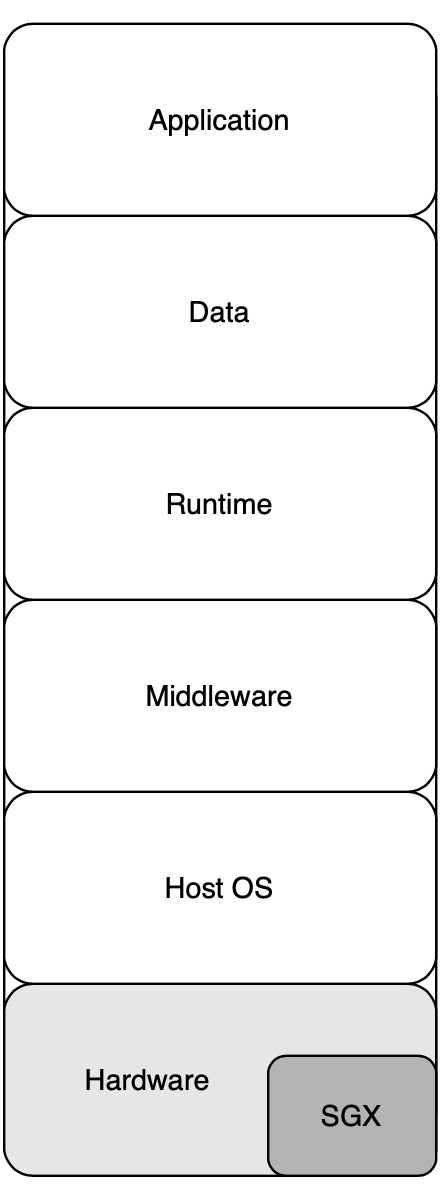
\includegraphics[width=0.2\linewidth]{IaaS_stack}}%
    \hspace{5em}
  \subcaptionbox{PaaS Stack\label{fig:saas_stack}}%
    {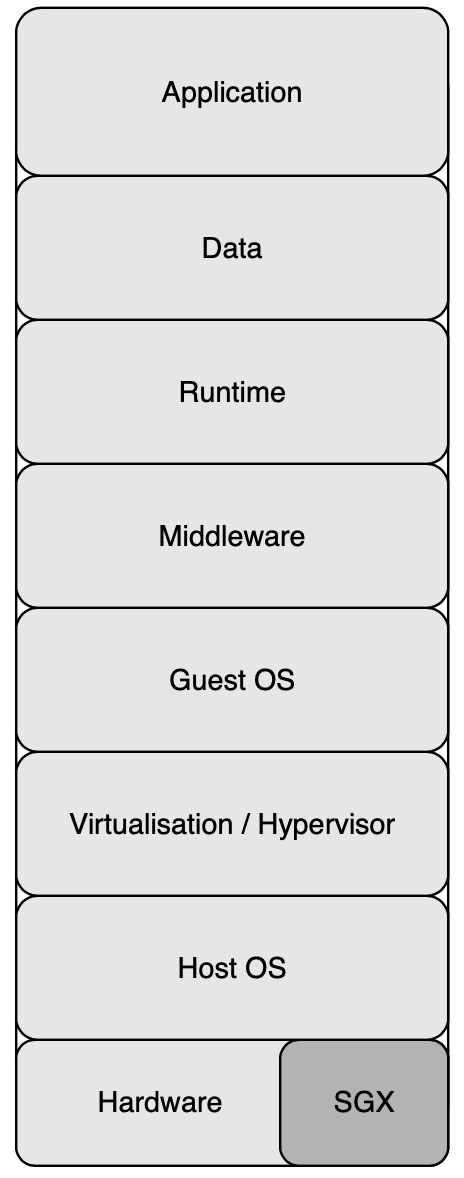
\includegraphics[width=0.2\linewidth]{SaaS_stack}}%
  \caption{Computing Stacks}
  \label{fig:computing_stacks}
\end{figure}

We will start development with a stack like figure \ref{fig:iaas_stack} as it is the simpler to customise and change to our needs especially for development. Everything besides the physical hardware can be customisable and it is managed by the user. In the end, we would like to expose the solution as a \gls{SaaS}, like figure \ref{fig:saas_stack} where it provides to the user a more abstracted environment, requiring less knowledge of computing bases and setups \cite{computing_stacks:1}.

As shown on figure \ref{fig:computing_stacks} and to achieve the objectives and goals of the project (\ref{sec:objectives_and_planned_contributions}), the hardware chosen was Intel's \gls{SGX} secure module. As explained in section \ref{ssec:intel_sgx}, this technology has the means and the ability to provide a truly isolated environment has required in this dissertation. The stack will be running a Linux Ubuntu Server \cite{ubuntu_server:1} operating system as the Host \gls{OS}, version 18.04 LTS. This version has compatibility with Intel's \gls{SGX} hardware, with the help of its \gls{SDK} and drivers \cite{sgx_sdk:1, sgx_drivers:1} and with some software needed in another layer of the stack.

Redis (v5.0.7 \cite{redis:1}) will be the key-value store application that will be worked on. This is the most used and most known \gls{KVS} technology, written in C language and will be deployed on the application component of the stack. To support large datasets, given \gls{SGX} limitations explained in section \ref{ssec:circumvention_of_sgx_limitations}, all data will be kept outside the enclave and will always be encrypted. The client can then decide to perform queries in encrypted form directly over the encrypted memory, sparing encryption and decryption cycles on the server. This will speed up the performance and will keep encryption keys away from the server in the cloud. Keys would be managed by the client which is considered trustable by the scope of this dissertation. Although this technique should help performance, it also means that system can lose some abilities and a set of operations. Fully homomorphic encryption is not feasible yet, so this solution will not be a full fledged solution. To this end, the solution will use the HomoLib, which is a JAVA Partial Homomorphic Cryptographic Library developed be the NOVA LINCS Research Center \cite{homolib:1}.

To help with \gls{SGX} integration a middleware software called Graphene \cite{graphene:1, graphene:2} will be used. This technology is a library \gls{OS} that \textit{"with \gls{SGX} support (...) can secure a critical application in a hardware-encrypted memory region. Graphene can protect applications from a malicious system stack with minimal porting effort"}. This library has already been tested with Linux Ubuntu Server 18.04 running as the \gls{OS}. 

Communications will be secure with the help of SGXStunnel \cite{sgxstunnel:1}, a prototype proxy to support TLS tunnelling with endpoints executed in a trusted execution environment provided by Intel SGX. \gls{SGX} termination means that at no time the data exchanged between the client and the server is exposed in clear text to any outsider because the packets are decrypted inside the secure module, which allows the network drivers, modules and physical cards to be removed from the \gls{TCB}.

Services and runtime environments will be coded using Java (Java SE 11 (LTS)) and the deployment of all softwares and services will be done with containers using docker technology \cite{docker:1}. Graphene already supplies integration with docker \cite{graphene_container:1}.

\section{Planned Testbench Environments} % (fold)
\label{sec:planned_testbench_environments}

The services will be deployed and tested in two different environments. The \textbf{development environment} translates to a local virtual machine that aims to simulate and be as close as possible to the production environment, but providing ease of development and rapid deployments. The \textbf{production environment} corresponds to a cloud provider that offers \gls{SGX} dedicated hardware, like OVHcloud \cite{ovhcloud:1}. The machines used should have the following specs:

\lstset{numbers=none, caption=Machine Specifications, label=lst:machine_specs}
\begin{lstlisting}
Dedicated Server Node
Processor: Intel 2x Xeon Silver 4214 - 24c/48t - 22.GHZ/3.2Ghz
Memory: 192 GB
Hard Drive: NVMe, SATA available
Public Network: Beginning at 1 Gbps
Private Network: Beginning at 2 Gbps
CloudLinux (Ubuntu 18.4 LTS Server 64 bits)
\end{lstlisting}

The tests will pe performed by a combination of the built-in Redis-Client benchmark tests \cite{redis_benchmark_cli:1} and to eliminate any bias claims, an external tester like the Yahoo! Cloud Serving Benchmark \cite{yahoo_benchmark:1}.

\section{Relevant Evaluation Criteria} % (fold)
\label{sec:relevant_evaluation_criteria}

The testers and benchmark clients will evaluate metrics that can be compared with a non secure solution. On the network layer, latency and throughput (as operations per seconds (ops/s)) and on the server side we will monitor the resources of the machines, like memory consumption, CPU load and also power consumption during the performance tests. Resource monitoring metrics should be gathered by the built in Linux tools like \textit{htop}, \textit{lsof} or \textit{vmstat}, and/or docker built-in tools like \textit{docker stats}.